\section{Gesamtsystem}\label{gesamtsystem}
In folgender Abbildung ist die Datenpipeline von dem Server des DWD bis zur Darstellung der Vorhersagen in der App zu sehen.  

\begin{figure}[htb]
 \centering
 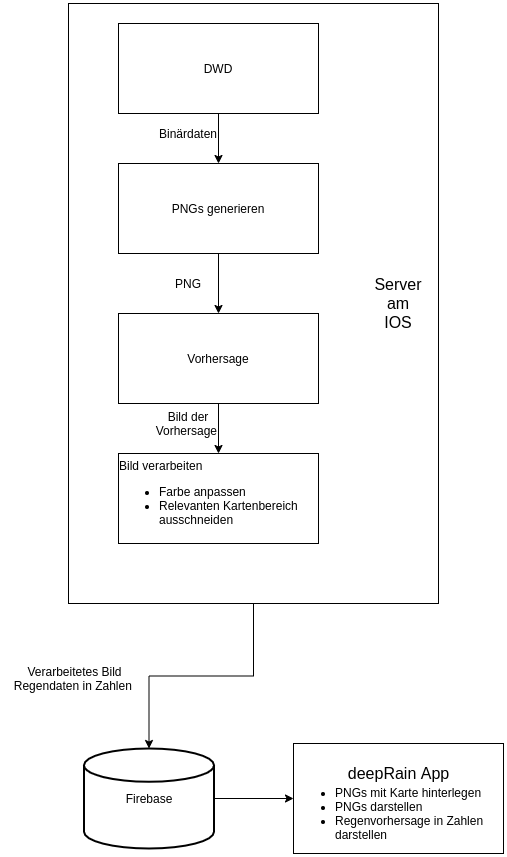
\includegraphics[width=0.6\textwidth,angle=0]{abb/Gesamtsystem}
 \caption[Das Gesamtsystem]{Das Gesamtsystem}
\label{fig:Beschreibung}
\end{figure}
\begin{sloppypar}
    \tolerance 9999
    \noindent
    Der DWD stellt alle fünf Minuten die neusten Regendaten für Deutschland im Binär Format auf dem Opendata Server des DWD zur Verfügung. 
    Diese werden heruntergeladen und in der Datenaufbereitung verwendet, um PNGs zu generieren (Siehe Kapitel \ref{die datenaufbereitung}). 
    Dieses PNGs werden im Anschluss verwendet, um eine Regenvorhersage zu machen (Siehe Kapitel \ref{die neuronalen netze}). 
    Der Output der Regenvorhersage ist wieder ein PNG. 
    Dieses PNG wird in der Firebase gespeichert und auf allen Geräten mit der installierten App angezeigt (Siehe Kapitel \ref{die deeprain app und das datenbankhandling}). 
    Der Übersichtlichkeit halber haben wir das gesamte Projekt in die drei Komponenten “Datenbeschaffung \& Vorverarbeitung”, “Vorhersage” und
    “App \& Datenbankhandling” aufgeteilt. 
    Die Komponente “Datenbeschaffung \& Vorverarbeitung” reicht vom Download der Binärdaten beim DWD bis zu den daraus generierten PNG’s. 
    In der Komponente “Vorhersage” werden die Regenvorhersage mithilfe von neuronalen Netzen gemacht. In der Komponente “App \& Datenbankhandling” 
    Geht es um das Datenmanagement mit der Firebase, und um die App, welche die Daten darstellt.
\end{sloppypar}